Multiple data sets were chosen to demonstrate the use of feature confidence level-sets proposed in this paper.
%
We defined a trait $T$ based on a priori knowledge of features of interest in the data.
%
While our study demonstrates feature confidence level-sets for univariate and bivariate data, the approach can be applied to higher dimensions.
%
Each variable is represented using a $mean$ and $SD$ field.
%
For each data set, we visualize the $ZLS_{T}$ individually and augmented with a single feature level-set $FLS_{T,K}$ for some level $K$ or a feature confidence level-set $FCLS_{T,C}$ for some confidence $C$ (and level $\epsilon$).

\begin{figure*}[!h]
\begin{subfigure}{0.195\linewidth}
\centering

\includegraphics[width=0.8\linewidth]{Images/Tangle/gt.pdf}
\vspace{-2mm}
\caption{Ground truth, $isoval=62$}
\label{fig:tangle_gt}
\end{subfigure}
\begin{subfigure}{0.195\linewidth}
\centering
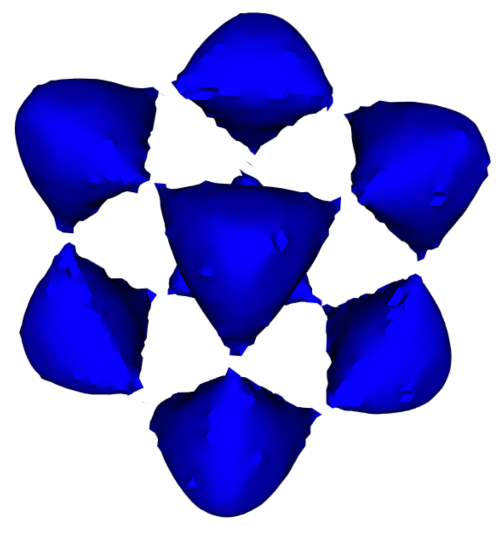
\includegraphics[width=0.8\linewidth]{Images/Tangle/zls.pdf}
\vspace{-2mm}
\caption{$ZLS_{T}$}
\label{fig:tangle_zls}
\end{subfigure}
\begin{subfigure}{0.195\linewidth}
\centering

\includegraphics[width=0.8\linewidth]{Images/Tangle/fls.pdf}
\vspace{-2mm}
\caption{$ZLS_{T}$ + $FLS_{T,2}$}
\label{fig:tangle_fls}
\end{subfigure}
\begin{subfigure}{0.195\linewidth}
\centering
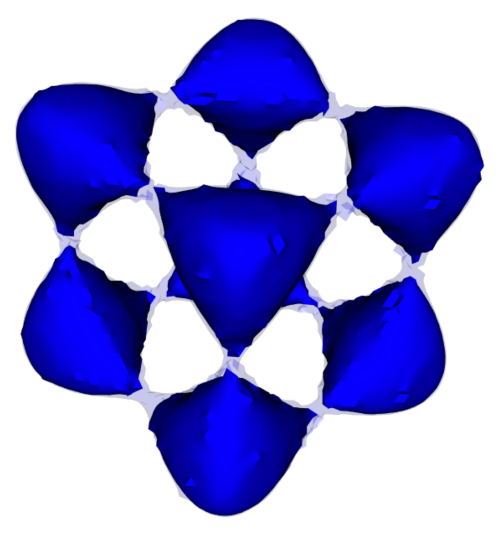
\includegraphics[width=0.8\linewidth]{Images/Tangle/fcls_68.pdf}
\vspace{-2mm}
\caption{$ZLS_{T}$ + $FCLS_{T,68\%}$}
\label{fig:tangle_fcls_68}
\end{subfigure}
\begin{subfigure}{0.195\linewidth}
\centering
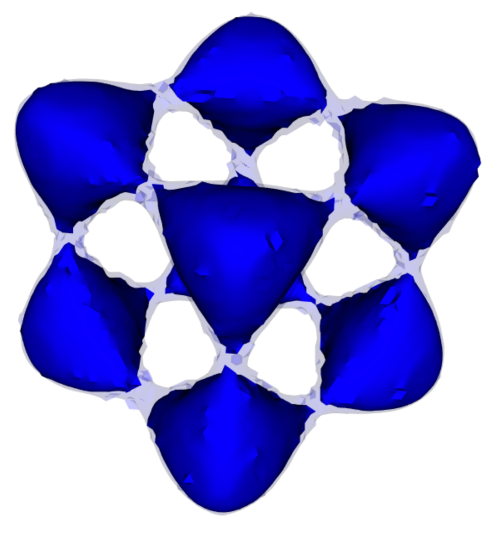
\includegraphics[width=0.8\linewidth]{Images/Tangle/fcls_95.pdf}
\vspace{-2mm}
\caption{$ZLS_{T}$ + $FCLS_{T,95\%}$}
\label{fig:tangle_fcls_95}
\end{subfigure}
\vspace{-2mm}
\caption{Visualization of sensitivity of the tangle function near values that form links between the multiple blobs. We use $T=[0,62]$.}
\vspace{-2mm}
\label{fig:tangle}
\end{figure*}

\begin{figure*}[h]
\begin{subfigure}{0.18\linewidth}
\centering
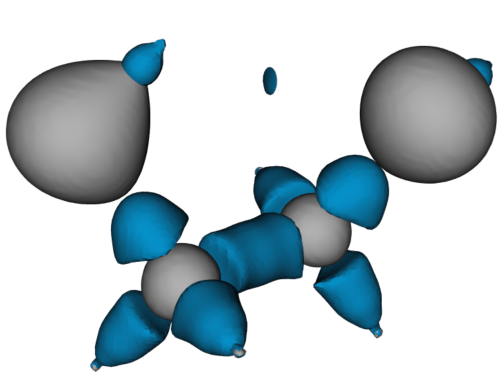
\includegraphics[width=\linewidth]{Images/EthaneDiol/gt.pdf}
\caption{$Rho_{isoval}=1.57$ (gray),\\ $s_{isoval}=-0.575$ (light blue)}
\label{}
\end{subfigure}
\begin{subfigure}{0.18\linewidth}
\centering
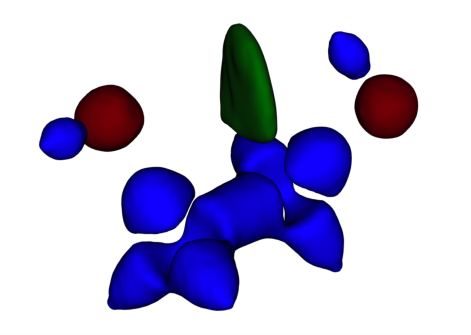
\includegraphics[width=\linewidth]{Images/EthaneDiol/zls_3.pdf}
\caption{$ZLS_{T}$}
\label{}
\end{subfigure}
\begin{subfigure}{0.18\linewidth}
\centering
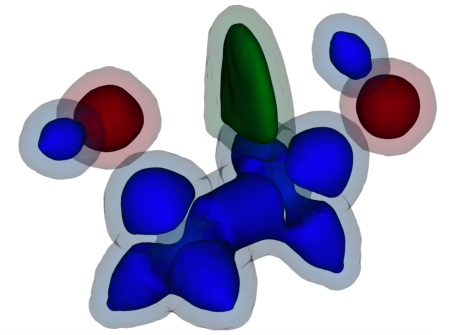
\includegraphics[width=\linewidth]{Images/EthaneDiol/fls_2_3.pdf}
\caption{$ZLS_{T}$ + $FLS_{T,2}$}
\label{}
\end{subfigure}
\begin{subfigure}{0.18\linewidth}
\centering
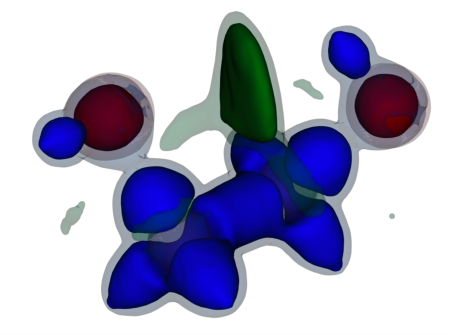
\includegraphics[width=\linewidth]{Images/EthaneDiol/fcls_68_3.pdf}
\caption{$ZLS_{T}$ + $FCLS_{T,68\%}$}
\label{}
\end{subfigure}
\begin{subfigure}{0.24\linewidth}
\centering
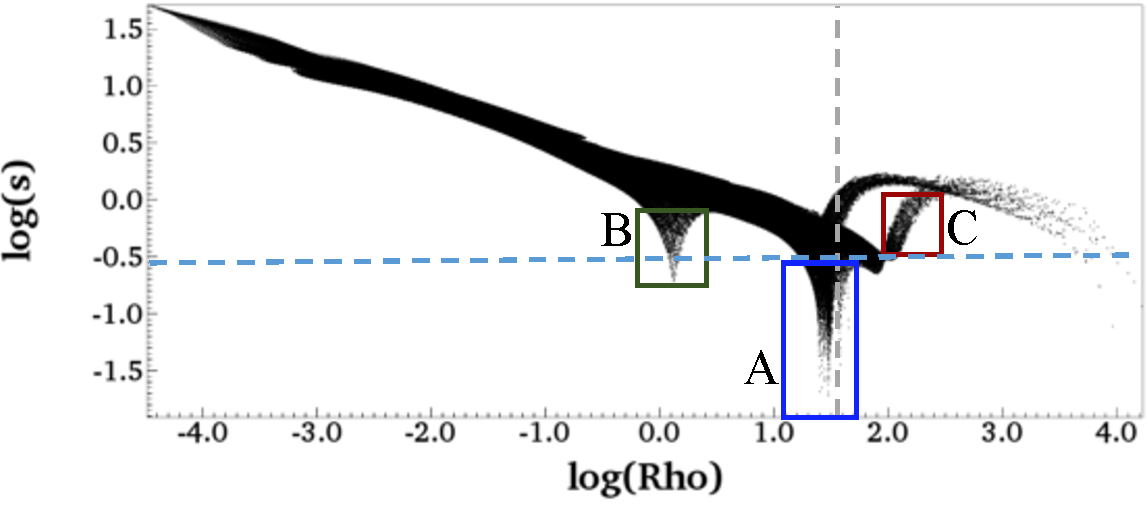
\includegraphics[width=\linewidth]{Images/EthaneDiol/scatterplot_3.pdf}
\caption{Attribute space 2D scatterplot, traits (labeled rectangular selections), and isovalues (dashed lines). We use $T = \left\{T_{A}, T_{B}, T_{C}\right\}$.} 
\label{}
\end{subfigure}
\caption{}
\label{}
\end{figure*}

